\documentclass{article}
\usepackage[utf8]{inputenc}
\usepackage{titlesec}
\usepackage{pgfplots}
\usepackage{enumitem}
\usepackage{array}



\title{Sample Exam}
\author{Payal Choudhary }
\date{\today}



\begin{document}

\maketitle
\begin{flushleft}
\large{Name: }\titlerule\\
\large{Roll Number: }\titlerule
\end{flushleft}
\vspace{1cm}

\begin{center}

\begin{tabular}{ | m{5em} | m{1cm}| m{1cm} | m{1cm} | m{1cm} | }
\hline
Question: & 1 & 2 & 3 & Total   \\ 
\hline
Points: & 10 & 10 & 0 & 20 \\ 
\hline
Bonus Points: & 0 &  5 & 10 & 15\\ 
\hline
Score: & & & & \\
\hline
\end{tabular}

\end{center}
\vspace{3cm}

\begin{center}
    

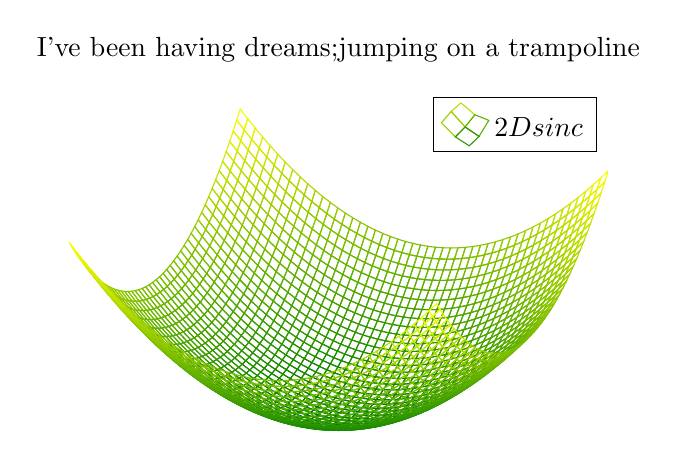
\begin{tikzpicture}
\begin{axis}[
    title=I've been having dreams;jumping on a trampoline,
    hide axis,
    colormap/greenyellow
    ,
]
\addplot3[
    mesh,
    samples=50,
    domain=-8:8,
]
{(x^2+y^2)};
\addlegendentry{$2D sinc$}
\vspace{1cm}
\end{axis}
\end{tikzpicture}
\end{center}


\begin{flushleft}

\begin{enumerate}
\item You need to use \textbf{pgfplot} to draw the figure. The source code for this plot is taken from an Overleaf
tutorial. Read the tutorial to learn about the functionality of pgfplot, you will eventually find the
relevant snippet.

\begin{enumerate}[label=(\alph*)]
\item(5 points)Play around with parameters to achieve this trampoline effect
\item(5 points)Change the title, and the colour scheme from the original
\end{enumerate}
\hfill{Total for Question 1: 10}

\item Read the caption to the figure.
\begin{enumerate}[label=(\alph*)]
\item(3 points) Which song is the caption taken from?
\item(2 points) This song is a duet. Who is the male vocalist?
\item (2 points) Which of the following was he associated with?\\
A. Led Zeppelin \hspace{0.5cm} B. Queen \hspace{0.5cm} C. One Direction \hspace{0.5cm} D. Nirvana
\item(3 points) Which of the following are Linkin Park songs?
\begin{list}{$\circ$}{}
\item Faint
\item Carnival of Rust
\item Enter Sandman
\item New Divide
\end{list}
\item(5 points (bonus)) In the above question, which artist(s) made the other song(s)?
\end{enumerate}
\hfill{Total for Question 2: 10}

\item(10 points (bonus)) Describe how Green Day’s American Idiot connects with the current sociopolitical
climate of the USA.




\end{enumerate}




\end{flushleft}

\end{document}